\clearpage
\item \points{20} {\bf A Simple Neural Network}

Let $X = \{x^{(1)}, \cdots, x^{(m)}\}$ be a dataset of $m$ samples with 2 features, i.e $x^{(i)} \in \mathbb{R}^2$. The samples are classified into 2 categories with labels $ y^{(i)} \in \{0, 1\}$. A scatter plot of the dataset is shown in Figure $\ref{fig:nn_plot}$:
	\begin{figure}[htbp] 
		\centering
		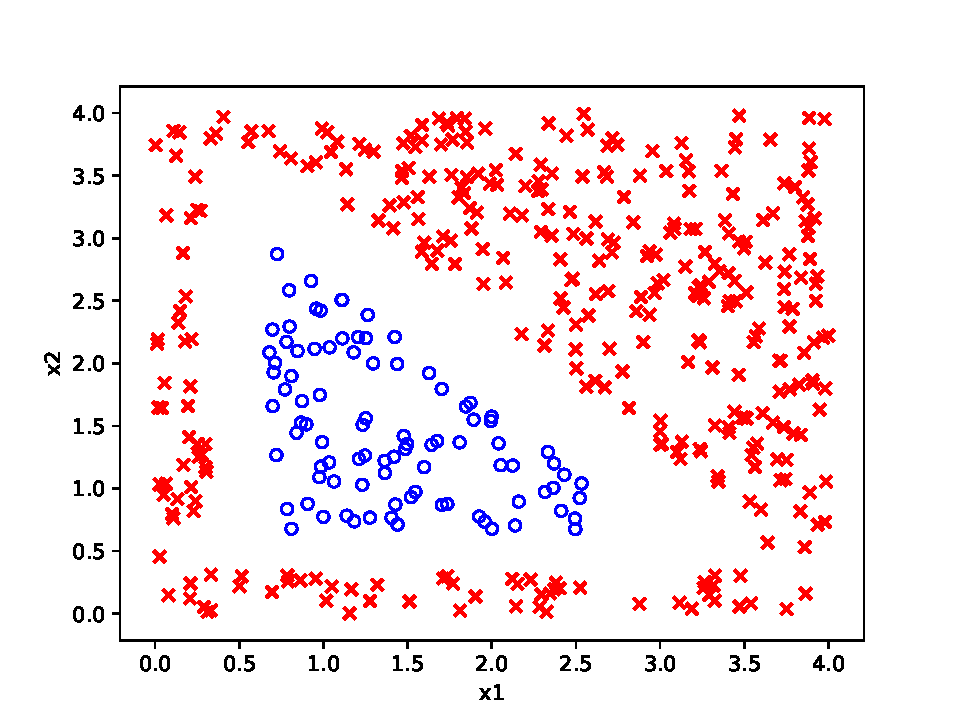
\includegraphics[scale=0.5]{../data/nn_plot.pdf}
		\caption{Plot of dataset $X$.}
		\label{fig:nn_plot}
	\end{figure}

	The examples in class $1$ are marked as as ``$\times$" and examples in class $0$ are marked as ``$\circ$". We want to perform binary classification using a simple neural network with the architecture shown in Figure $\ref{fig:nn_arc}$:
	\begin{figure}[htbp]
		\centering
		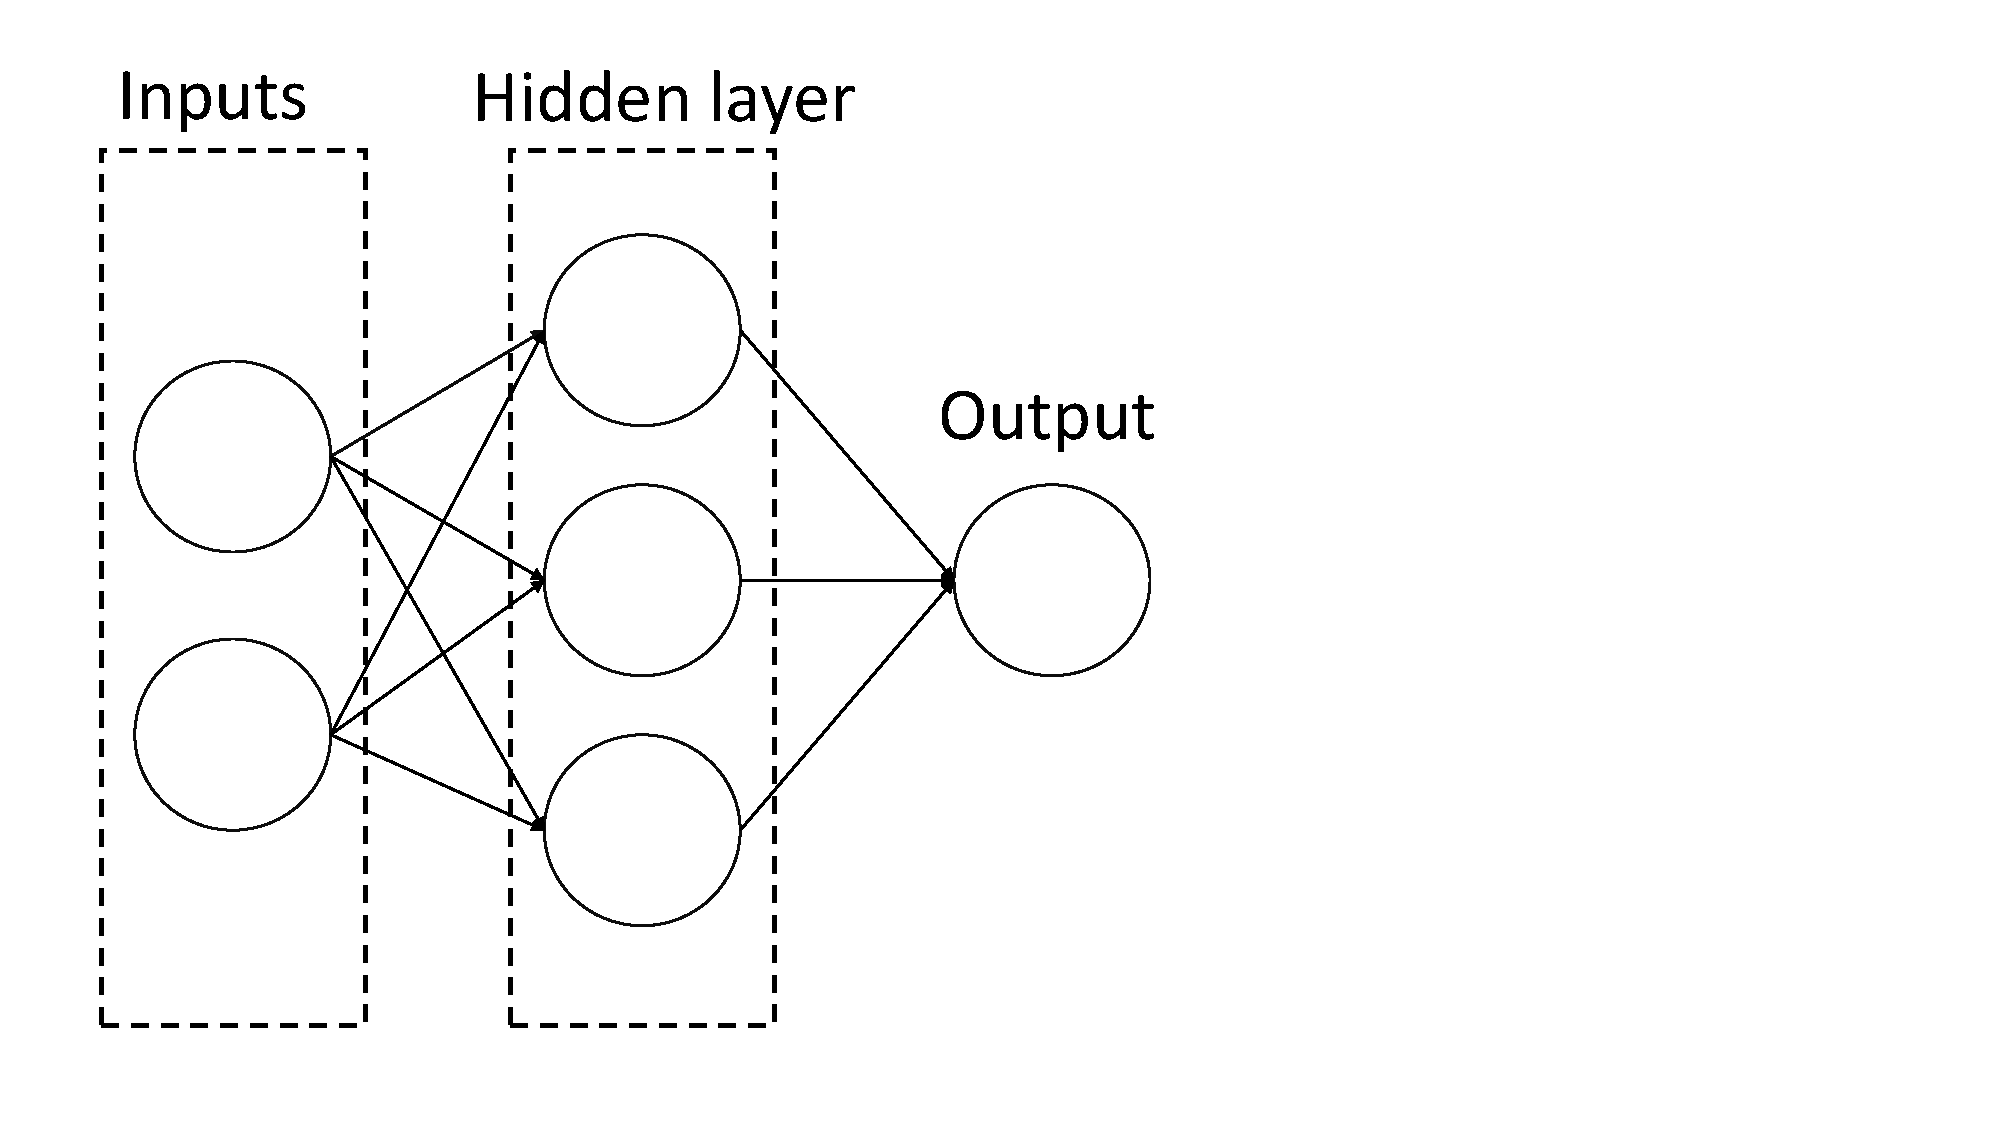
\includegraphics[scale=0.2, trim = 0 0 360 0, clip]{../data/nn_architecture.pdf}
		\caption{Architecture for our simple neural network.}
		 \label{fig:nn_arc}
	\end{figure}

	Denote the two features $x_1$ and $x_2$, the three neurons in the hidden layer $h_1, h_2$, and $h_3$, and the output neuron as $o$. Let the weight from $x_i$ to $h_j$ be $w_{i, j}^{[1]}$ for $i \in \{1, 2\}, j \in \{1, 2, 3\}$, and the weight from $h_j$ to $o$ be $w_{j}^{[2]}$. Finally, denote the intercept weight for $h_j$ as $w_{0, j}^{[1]}$, and the intercept weight for $o$ as $w_{0}^{[2]}$. For the loss function, we'll use average squared loss instead of the usual negative log-likelihood:
  $$l = \frac{1}{m}\sum_{i=1}^{m}(o^{(i)} - y^{(i)})^2,$$
  where $o^{(i)}$ is the result of the output neuron for example $i$.

\begin{enumerate}

  \item \subquestionpoints{5} Suppose we use the sigmoid function as the activation function for $h_1, h_2, h_3$ and $o$.
      What is the gradient descent update to $w_{1, 2}^{[1]}$, assuming we use a learning rate of $\alpha$?
      Your answer should be written in terms of $x^{(i)}$, $o^{(i)}$, $y^{(i)}$, and the weights.\\
      
\ifnum\solutions=1 {
  \begin{answer}
 \end{answer}

} \fi


  \ifnum\solutions=1 {
  \clearpage
} \fi
\item \subquestionpoints{10} Now, suppose instead of using the sigmoid function for the activation function
      for $h_1, h_2, h_3$ and $o$,
      we instead used the step function $f(x)$, defined as
		\begin{align*}
		f(x) = \begin{cases}
		1, x \ge 0 \\
		0, x < 0
		\end{cases}
		\end{align*}

Is it possible to have a set of weights that allow the neural network to classify this dataset with 100\% accuracy?

If it is possible, please provide a set of weights that enable 100\% accuracy by completing \texttt{optimal\_step\_weights} within \texttt{src/p01\_nn.py} and explain your reasoning for those weights in your PDF.

If it is not possible, please explain your reasoning in your PDF. (There is no need to modify \texttt{optimal\_step\_weights} if it is not possible.)


\textbf{Hint:} There are three sides to a triangle, and there are three neurons in the hidden layer.

\ifnum\solutions=1 {
  \begin{answer}
 \end{answer}

} \fi

  
  \ifnum\solutions=1 {
  \clearpage
} \fi
\item \subquestionpoints{10} Let the activation functions for $h_1, h_2, h_3$ be the linear function $f(x) = x$ and the activation function for $o$ be the same step function as before.

Is it possible to have a set of weights that allow the neural network to classify this dataset with 100\% accuracy?

If it is possible, please provide a set of weights that enable 100\% accuracy by completing \texttt{optimal\_linear\_weights} within \texttt{src/p01\_nn.py} and explain your reasoning for those weights in your PDF.

If it is not possible, please explain your reasoning in your PDF. (There is no need to modify \texttt{optimal\_linear\_weights} if it is not possible.)


\ifnum\solutions=1 {
  \begin{answer}
Even though there are two layers (hidden layer and output layer) in our neural network, without a non-linear activation function, our neural network is equivalent to a linear function.\\
Assume $o = step(z)$, where $step$ is the step function. So, $z$ can be written as a linear function of $x$: $$z = w^{[2]}_0+\sum\limits_{i=1}^3 w^{[1]}_{0,i} w^{[2]}_{i} + (\sum\limits_{i=1}^3 w^{[1]}_{1, i} w^{[2]}_{i}) x_1 + (\sum\limits_{i=1}^3 w^{[1]}_{2, i} w^{[2]}_{i}) x_2$$. In conclusion, the decision boundary is only a straight line. It's impossible to have a set of weights that allow the neural network to classify this dataset with 100\% accuracy?
\end{answer}

} \fi


\end{enumerate}
